% !TeX spellcheck = ru_RU
%pdflatex, utf8
\documentclass[unicode, 10pt, a5paper, oneside]{article}

% Установка полей страницы
%\usepackage{anysize}
%\marginsize{0.3cm}{0.3cm}{0.3cm}{0.3cm}
\usepackage[a5paper, margin=0.3cm, bindingoffset=0cm]{geometry}

% Поддержка русского языка
\usepackage[T2A]{fontenc}		% Корректная кодировка шрифта при использовании cm-super
\usepackage[utf8]{inputenc}		% Кодировка ввода
\usepackage[russian]{babel}		% Словарь расстановки переносов
%\usepackage{cmap}				% Перекодировка символов в pdf при использовании обычного cm

% Всякие математические фишки
\usepackage{amsmath}
\usepackage{amsfonts}
\usepackage{amssymb}

% Изменение цвета, работа с графикой
\usepackage{color}
\usepackage[pdftex]{graphicx}
\graphicspath{{images/}}

% Команда для вставки ссылок \url{URL}
\usepackage[hyphens]{url}
\urlstyle{rm}					% Стиль шрифта ссылок: с засечками

% Кликабельные ссылки внутри документа
\usepackage[unicode]{hyperref}

% Включает отступ у первого абзаца в разделе
\usepackage{indentfirst}

% Настрйока стиля списков
\usepackage{enumitem}
\setlist{noitemsep, leftmargin=*, labelindent=\parindent, topsep=0pt, parsep=0pt, partopsep=0pt}

\setlist[itemize,1]{label=$\diamond$}
\setlist[itemize,2]{label=\textendash}
\setlist[itemize,3]{label=$\star$}

\renewcommand{\alph}[1]{\asbuk{#1}} % Костыль для кирилической нумерации вместо латинской
\setlist[enumerate,1]{label=\arabic*)}
\setlist[enumerate,2]{label=\alph*)}
\setlist[enumerate,3]{label=(\arabic*)}


\usepackage{textcomp}			% Команды для вставки разных символов (градусы, проценты, итд)
\usepackage{float}				% Размещение плавающих объектов там где они созданы (X)
\usepackage{wrapfig}			% Обтекаемые текстом рисунки

% Подписи у флоатов
\setlength{\intextsep}{0pt} % Отстут вокруг плавающих окружений
\usepackage{caption}
\captionsetup{parskip=0pt}
\captionsetup[figure]{labelsep=period,justification=centering,singlelinecheck=false,textfont=small,labelfont=small,aboveskip=2pt,belowskip=0pt}

% Изменение формата заголовков разделов
\usepackage{titlesec}
\titleformat{\section}{\newpage\small\bfseries}{\thesection. }{0pt}{}{}
\titlespacing*{\section}{0pt}{0pt}{0pt}

\titleformat{\subsection}{\small\bfseries}{\thesubsection. }{0pt}{}{}
\titlespacing*{\subsection}{0pt}{0pt}{0pt}

\usepackage{array}				% Позволяет объявить свои типы колонок
\usepackage{calc}				% Математика, исп-ся для расчёта ширины колонки
\usepackage{longtable}			% Длинные таблицы

% Минимальный отступ в таблицах
\setlength{\tabcolsep}{1.5mm}

% Новые типы колонок. Ширина задётся как доля от linewidth
\newcolumntype{L}[1]{p{#1\linewidth-2\tabcolsep-2\arrayrulewidth}}
\newcolumntype{C}[1]{>{\centering}p{#1\linewidth-2\tabcolsep-2\arrayrulewidth}}
\newcolumntype{R}[1]{>{\raggedleft}p{#1\linewidth-2\tabcolsep-2\arrayrulewidth}}
\newcolumntype{U}[2]{p{#1\linewidth-(#2)}}

% Стараться не оставлять одиноких строк в начале и конце абзаца
\clubpenalty=1000
\widowpenalty=1000

% Расстановка отступов и переносов
\emergencystretch=2.5em			% Максимальный промежуток между словами
\tolerance=2000
\frenchspacing


\begin{document}

\setcounter{section}{120}

% Вопрос 121 ----------------------------------------------------------
\section{Основные понятия процесса проектирования систем управления. Цель процесса проектирования.}

Цель процесса проектирования состоит в том, чтобы на основе априорной информации и апостериорной информации, получаемой в процессе проектирования, разработать техническую документацию, требуемую для изготовления объекта.

Процесс проектирования --- это процесс создания объекта, прототипа или прообраза необходимого для его изготовления. 

Проектирование средств управления по существу представляет собой процесс управления с обратной связью.

Техническое задание формирует входные данные или установки, которые сравниваются с результатами проектирования и, если они не совпадают, то цикл проектирования повторяется пока ошибка не будет в допустимых пределах.

Кроме этого процесс проектирования можно представить в виде графа. Принимая точку 0 за формулировку проблемного варианта ее решение можно представить отрезками а1, а2, а3, каждому варианту соответствует несколько проблем Wi.
Выбор вариантов аi является творческим, трудно формализуемым процессом.

\begin{figure}[H]
\centering
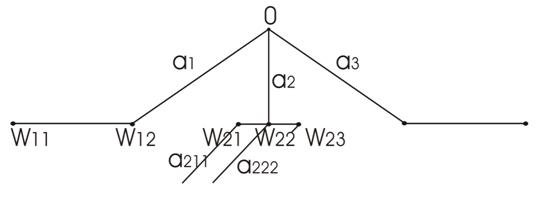
\includegraphics[width=0.5\textwidth]{121.jpg}
\caption{Граф процесса проектирования}
\end{figure}

В настоящее время, автоматизированное проектирование средств управления связано с новым этапом развития --- это САПР САУ, предназначенных для решения задач научно-исследовательского, эскизного и частично технического проектирования. Согласно определению, рекомендуемому ГОСТом, АП --- это комплекс программно-технических взаимосвязанных с необходимыми подразделениями проектной организации.

С точки зрения управления САПР АСУТП сама является АСУТП.

% Вопрос 122 ----------------------------------------------------------
\section{Системный подход к проектированию.}

Основной общий принцип системного подхода заключается в рассмотрении частей явления или сложной системы с учетом их взаимодействия.	Системный подход включает в себя:
\begin{enumerate}
\item выявление структуры системы,
\item типизацию связей,
\item определение атрибутов,
\item анализ влияния внешней среды.
\end{enumerate}

В технике дисциплину, исследующую сложные технические системы, называют системотехникой.

Конкретизация системного подхода привела к появлению следующих вариантов:
\begin{enumerate}
\item Структурный подход --- при нем требуется синтезировать варианты системы из компонентов или блоков и оценивать варианты при их частичном 
переборе с предварительным прогнозом характеристик;
\item Блочно-иерархический. Используются идеи декомпозиции сложных описаний объектов и соответственно средств их создания на иерархическом условии взаимосвязи между собой;
\item Объектно-ориентированный --- состоит из структурных принципов, используемых при разработке информационных систем. Прежде всего это ПО.
\end{enumerate}

Ряд важных структурных принципов, используемых при разработке ПО, выражен в объектно-ориентированном подходе.
  
Преимущества последнего подхода:
\begin{enumerate}
\item вносит в модель определенность
\item cокращает объем спецификации
\item уменьшает вероятность искажения результата.
\end{enumerate}

Для всех подходов характерны следующие особенности:
\begin{enumerate}
\item Структуризация процесса проектирования, выражаемая декомпозицией проектной задачи и документацией на стадиях и этапах.
\item Итерационный характер проектирования.
\item Типизация и унификация проектных решений и средств проектирования.
\end{enumerate}

% Вопрос 123 ----------------------------------------------------------
\section{Структура процесса автоматизированного проектирования.}

При использовании блочно-иерархического подхода к проектированию представление о проектировании расчленяют на иерархические уровни. Список уровней в каждом приложении могут быть специфическими, но для большинства характерны три крупных уровня:

\begin{enumerate}
\item Системный. Разработка структурных схем, планов и т.д.
\item Макроуровень. Функциональные, принципиальные, кинематические схемы.
\item Микроуровень. Проектирование отдельных деталей.
\end{enumerate}

Наряду с декомпозицией описаний на иерархическом уровне применяется разделение представлений о проектируемых объектах на аспекты. Аспект описания (страта) --- описание системы или ее части с нею оговоренной точки зрения определяемой функциональными физическими или иного типа соотношениями между свойствами и отношениями.

Обычно различают аспекты: 
\begin{itemize}
\item Функциональный;
\item Информационный;
\item Структурный;
\item Поведенческий.
\end{itemize}

Стадии проектирования --- это части проектирования, как процесса, развивающиеся во времени. Различают стадии:
\begin{itemize}
\item научно-исследовательскую (НИР),
\item эскизного проекта,
\item технического,
\item рабочего,
\item испытание опытных образцов и партий.
\end{itemize}

Разработку ТЗ называют внешним проектированием, а реализацию ТЗ --- внутренним.

Основное содержание ТЗ:

\begin{itemize}
\item Назначение объекта;
\item Условие эксплуатации (допуски);
\item Требования к входным параметрам (т.е. к величинам характеризующим свойства объектов).
\end{itemize}

Эти требования выражаются в виде условий работоспособности.

% Вопрос 124 ----------------------------------------------------------
\section{Основные типы автоматизированных систем, разновидности САПР.}

Достижение поставленных целей на современных предприятиях выпускающих сложные изделия невозможно без применения автоматизированных систем. Специфика задач, решаемых на различных этапах жизненного цикла, обуславливается разнообразием применяемых автоматизированных систем.

\begin{figure}[H]
\centering
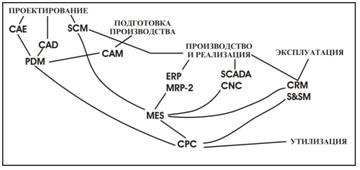
\includegraphics[width=0.5\textwidth]{124.jpg}
\caption{Основные типы автоматизированных систем}
\end{figure}

Основные типы автоматизированных систем с привязкой к жизненному циклу :

\begin{itemize}
\item CAE --- это системы расчетов и инженерного анализа.
\item CAD --- это системы конструкторского проектирования.
\item CAM --- это системы технологической подготовки производства.
\item PDM --- системы управления проектными данными CAE, CAD, CAM.
\item SCM --- системы управления цепочками поставок.
\end{itemize}

Информационная поддержка этапа производства продукции осуществляется АСУТП. К АСУТП относятся системы планирования и управления предприятиями (EPR) и системы планирования производства и требования к материалам MPR-2, а так же производственные исполнительные системы MES  и системы управления взаимоотношениями с заказчиками CRM.

Маркетинговые задачи возлагаются на системы S\&SN, которые используются так же и для обслуживания изделий.

Для выполнения диспетчерских функций (сбор, обработка данных) о состоянии оборудования и техпроцесса, разработки программного обеспечения для встроенного оборудования АСУТП используются системы SCADA. Непосредственное программное управление оборудованием осуществляется с помощью системы CNC на базе контроллеров встроенных в техническое оборудование. CPC --- это система электронного бизнеса для управления данными в интегрированном информационном пространстве. Характерная ее особенность это обеспечение взаимодействия предприятий.

\underline{Структура САПР}

САПР состоит из проектировочных и обслуживающих подсистем.

Структурирование САПР по различным аспектам обуславливает появление видов обеспечения САПР:
\begin{enumerate}
\item техническое --- включающее ЭВМ, периферию, сетевое оборудование и измерительные средства;
\item математическое обеспечение --- это матмодели, методы;
\item программное;
\item информационное (СУБД);
\item лингвистическое, выраженное языками общения между проектировщиками и ЭВМ, языками программирования и языками обмена данными между техническими системами;
\item методическое, включающее методики проектирования;
\item организационные.
\end{enumerate}

Разновидности САПР:

I. По приложениям различают:
\begin{itemize}
\item для машиностроения MCAD
\item для электроники ECAD (EDA)
\item в области архитектуры и строительства
\end{itemize}

II. По характеру базовой системы:
\begin{itemize}
\item САПР на базе машинной графики и геометрического моделирования
\item САПР на базе СУБД
\item САПР на базе конкретного прикладного пакета (CAE), примером является MATHCAD, MALAB
\item Комплексные САПР.
\end{itemize}

% Вопрос 125 ----------------------------------------------------------
\section{Стадии проектирования автоматизированных систем и аспекты их описания.}

При проектировании сложных систем выделятся следующие стадии:

\begin{enumerate}
\item Стадия предварительного проектирования, или стадия научно-исследовательских работ, связана с поиском принципиальных возможностей построения систем, исследованием новых принципов, структур, технических средств, обоснованием наиболее общих решений; результат --- техническое предложение.
\item Стадия эскизного проектирования или опытно-конструкторских работ --- производится детальная проработка всех частей проекта, конкретизируются и детализируются  технические решения. 
\item Стадия рабочего проекта --- формируется вся необходимая документация для изготовления изделия. Далее создаётся и испытывается опытный образец (или партия изделия), по результатам испытаний вносятся необходимые коррективы в проектную документацию, после чего осуществляется внедрение. 
\end{enumerate}
 
Этап проектирования --- составная часть любой из стадий  проектирования, сводящихся выполнению операций и процедур, которые относятся к одному аспекту или иерархическому уровню. 

Проектное решение --- промежуточное или конечное описание объекта, необходимое и достаточное для рассмотрения и определения дальнейшего направления или окончания проектирования. 

Проектная процедура --- формализованная совокупность действий, выполнения которых оканчивается проектным решением (оформление чертежа изделия, расчёт его параметров). 

Проектная операция --- действие или формализованная совокупность действий, составляющих часть проектной процедуры, алгоритм которых остаётся неизменным для ряда проектных процедур (вычерчивание типового графического изображения --- колеса, вала; решения системы уравнений и т.п.). 

Маршрут  проектирования --- последовательность этапов и/или проектных процедур. 

Расчленение (декомпозиция) описаний по характеру отображаемых свойств объекта приводит к появлению ряда аспектов описания:

\begin{enumerate}
\item Функциональный аспект связан с отображением основных принципов функционирования, характера физических и информационных процессов, протекающих в объекте. 
\item Конструкторский аспект связан с реализацией результатов функционального проектирования, то есть с определением геометрических форм объектов и их взаимным расположением в пространстве. 
\item Технологический аспект относится к реализации результатов конструкторского проектирования, то есть связан с описанием средств и методов изготовления объектов.
\end{enumerate}
 
Возможно более дифференцированное описание свойств объекта с выделением в нём ряда подсистем и соответствующего числа аспектов (например, функциональный аспект можно разделить по физическим основам описываемых явлений на аспекты электрических, механических, гидравлических, химических и т.д.).

Следует отметить, что понятие аспекта уровня проектирования относится к структурированию представлений о проектируемом объекте, а понятие этапа --- к структурированию процесса проектирования. 

По характеру и степени участия человека и использования ЭВМ различают несколько режимов проектирования.

Автоматический режим имеет место при выполнении маршрута проектирования и формальным алгоритмом на ЭВМ без вмешательства человека в ход решения. Ручной режим характеризуется выполнением маршрута без помощи ЭВМ. Автоматизированное проектирование является частично автоматизированным, если часть проектных процедур выполняется человеком, а часть --- с использованием ЭВМ. 

Диалоговый (интерактивный) режим является более совершенным режимом, при нём все процедуры в маршруте выполняются с помощью ЭВМ, а участие человека проявляется в оперативной оценке результатов проектных процедур или операций, в выборе  продолжений и корректировке хода проектирования.

Развитие САПР происходит, в частности, в направлении движения степени автоматизации. Однако работа в режиме диалога необходима, поскольку полностью процесс проектирования сложных систем формализовать не удаётся, а участие человека в ряде случаев позволяет ускорить процесс принятия решений.

% Вопрос 126 ----------------------------------------------------------
\section{Особенности проектирования САПР.}

Имеется два этапа направления деятельности при создании автоматизированных систем:

\begin{enumerate}
\item Проектирование автоматизированных систем конкретными предприятиями на базе готовых программных и аппаратных компонентов --- \underline{системная интеграция};
\item Проектирование автоматизированных систем, ориентированных на многократное использование --- \underline{компонентно-ориентированная разработка} Это направление относится к области разработки математического и программного обеспечения для реализации функций автоматизированной системы..
\end{enumerate}

Автоматизированные системы и компоненты автоматизированных систем являются сложным комплексом и при их проектировании используются несколько стилей:

\begin{enumerate}
\item нисходящее проектирование;
\item восходящее проектирование;
\item эволюционное проектирование.
\end{enumerate}

Этапы нисходящего проектирования:

\begin{enumerate}
\item Верхний уровень --- концептуальное проектирование. Выполняется в процессе предпроектных решений и ТЗ. Предпроектные исследования проводят путем анализа деятельности предприятия. На основе анализа результата строят модель. Далее разрабатывают исходную концепцию которая включает в себя предложения по изменению структуры предприятия. Эскизный проект представляют в виде проектной документации. После этого разрабатывают прототип. Прототип представляет собой набор программ эмулирующих работу системы.
\item Содержание последующих этапов нисходящего проектирования является уточнением перечня приобретаемого оборудования и готовых программных продуктов и т.п. и эти работы составляют рабочее проектирование.
\end{enumerate}

% Вопрос 127 ----------------------------------------------------------
\section{Понятие о CALS-технологиях.}

CALS-технологии (Continious Aquisition and Lifecycle Control) --- это технологии комплексной компьютеризации сфер промышленного производства цель которых унификация и стандартизация спецификаций промышленной продукции.

Цель --- сокращение объемов проектных работ.

В CALS системах предусмотрено хранение, обработка, передача информации в компьютерных средах.
Применение CALS технологий позволяет существенно сократить объемы проектных работ, так как описания хранятся в унифицированных форматах данных сетевых серверов.

Развитие CALS технологий, по мнению ученых всего мира, должно привести к появлению виртуальных производств. Среди несомненных достижений CALS технологий следует отметить распространение передовых проектных решений и возможность многократного воспроизведения частей проекта в новых разработках. Главная проблема построения открытых распределенных автоматизированных систем управления --- это обеспечение единообразного описания и интерпретации данных. Важная проблема, требующая решения при создании комплексных САПР --- это управление сложностью проекта и интерпретация программного обеспечения. Эти проблемы включают в себя декомпозиции проектов, распараллеливание проектных работ и создание межпрограммных интерфейсов.

Неотъемлемым свойством CALS является информационная интеграция, когда одна и та же конструкторская документация может быть использована в разных проектах, а технологическая --- адаптирована к разным производственным условиям.

% Вопрос 128 ----------------------------------------------------------
\section{Открытые системы.}

Одной из главных тенденций современной индустрии информационных систем является создание открытых систем, то есть имеющих свойство мобильности программного обеспечения на различные аппаратные платформы и свойство приспособляемости системы к ее модификации. Открытость системы подразумевает выделение в системе интерфейсной части. Значительное развитие концепции открытости получило в области построения вычислительных сетей, поддерживаемых международными стандартами. Идея открытости широко поддерживается при построении программного, информационного и лингвистического обеспечения автоматизированных систем. В результате повышения универсальности программ и расширяются возможности их адаптации к конкретным условиям.

Основные аспекты открытости отражены в следующих стандартах:

\begin{enumerate}
\item API --- интерфейсы прикладных программ с операционным окружением
\item Стандарты межпрограммных интерфейсов, включая языки программирования
\item Стандарты сетевого взаимодействия
\item Стандарты пользовательского интерфейса
\item Стандарты средств защиты информации
\end{enumerate}

Группы стандартов: ISO, IEEE, EIA, POSIX.

Профилем открытой системы называется совокупность стандартов и других нормативных документов, обеспечивающая выполнение системой заданных функций.

% Вопрос 129 ----------------------------------------------------------
\section{Техническое обеспечение систем автоматизированного проектирования.}

Используемые в САПР технические средства должны обеспечивать:

\begin{enumerate}
\item выполнение проектных процедур для которых имеется программное обеспечение;
\item обеспечить поддержку интерактивного режима работы;
\item обеспечить взаимодействие между проектировщиками.
\end{enumerate}

АРМ --- автоматизированное рабочее место --- рабочие места проектировщиков (узлы), связанные между собой средой передачи данных.

Среда передачи данных представлена каналами передачи данных, состоящих из линий связи и коммутационного оборудования (витая пара, коаксиальный кабель, волоконно-оптическая связь).

Разделяют оконечное оборудование данных, выполняющее определенную работу по проектированию, и аппаратуру окончания канала данных, служащую ля связи оконечного оборудования данных со средой передачи данных.

Имеется 2 метода разделения линии передачи данных --- TDM и FDM --- Time и Frequency Division Method, то есть временное и частотное мультиплексирование.

% Вопрос 130 ----------------------------------------------------------
\section{Типы сетей, методы доступа в сетях, протоколы и стеки протоколов в вычислительных сетях.}

Сети подразделяются на:

\begin{enumerate}
\item локальные
\item корпоративные
\item территориальные (различают: магистральные каналы передачи данных, обслуживанием занимаются провайдеры, которые представляют коммутационные услуги многим пользователям)
\item глобальные
\end{enumerate}

Типичная структура крупных корпоративных сетей САПР --- это "клиент-сервер". Сети клиент-сервер подразделяют:

\begin{enumerate}
\item файл-сервер
\item серверы баз данных автоматизированных систем
\item серверы приложений
\item коммутационные серверы
\item специализированные серверы
\end{enumerate}

Наряду с архитектурой клиент-сервер применяются одноранговые сети в которых любой узел, в зависимости от решаемой задачи, может выполнять функции как сервера так и клиента.

В соответствии со способами коммутации сети различают сети с коммутацией каналов и сети с коммутацией пакетов.

Для удобства модернизации сложных информационных систем их делают открытыми. Реализация концепции открытости привела к появлению эталонной модели взаимосвязи открытых систем ЭМВОС (OSI). В ней даны основные принципы, общие правила и соглашения обеспечивающие взаимодействие информационных систем, которые называются протоколами.

Различают семь уровней ЭМВОС:
\begin{itemize}
\item физический
\item канальный
\item сетевой
\item транспортный
\item сеансовый
\item представительный 
\item прикладной
\end{itemize}

Методы доступа в ЛВС:
\begin{enumerate}
\item Множественный доступ с контролем несущей и обнаружением конфликтов МДКН/ОК (CSMA/CD) --- основан на контроле наличия электрических колебаний и устранения конфликтов путем повторения захвата линии через определенные моменты времени
\item Маркерный метод доступа --- основан на передаче полномочий передатчика с помощью специального информационного объекта --- маркера.
\end{enumerate}

Структура кадра МДКН/ОК:
\begin{itemize}
\item Преамбула --- 7 байт
\item Ограничитель --- 1 байт
\item Адрес назначения --- 2 или 6 байт
\item Адрес источника --- 2 или 6 байт
\item Длина кадра --- 2 байта
\item Данные --- от 64 до 1518 байт
\item Заполнение и контрольный код --- 4 байта
\end{itemize}

Стек протоколов TCP/IP.

\begin{enumerate}
\item TCP/IP --- 5-уровневые протоколы, основанные на протоколе транспортного уровня TCP и протоколе сетевого уровня  IP. TCP --- транспортный, дуплексный протокол с установкой соединения. Протокол является байтовым, т.е. каждый байт имеет свой порядковый номер.
\item IP --- это сетевой протокол дейтограммный, без установления соединения. Дейтограмма --- это пакет, передаваемый независимо от других частей одного и того же сообщения с коммутацией пакетов. К основным функциям IP протокола относят: фрагментацию и сборку пакетов имеющих другие протоколы. Максимальная пропускная способность TCP/IP --- $2^{32}$ байт/ время жизни дейтограммы.
\item UDP --- user datagram protocol --- транспортный протокол без установления соединения. Используется чаще всего для сообщения, помещающегося в один пакет.
\item SMTP --- simple mail transport protocol --- почтовый протокол прикладного уровня
\item FTP --- file transport protocol --- протокол с функциями представительного уровня
\item Telnet --- протокол с функциями сеансового уровня
\end{enumerate}

В сетях TCP/IP за управляющие функции сетевого уровня отвечает протокол ICMP, а за мониторинг состояния сети --- SNMP (simple network management protocol).

% Вопрос 131 ----------------------------------------------------------
\section{САПР систем управления.}
Изучение поведения и конструирование систем управления, обладающих требуемыми в приложениях свойствами, является ключевой задачей теории управления. При этом на первый план выдвигаются такие свойства систем, как устойчивость, оптимальность, поведение в присутствии неопределенных помех и т. д. 

Для описания одной и той же реальной системы может быть использован разный математический аппарат, который зависит от целей исследования и требований точности и адекватности. Именно математическое описание будет определять выбор инструментальных средств и технологий проектирования систем. При этом на современном этапе особое внимание уделяется проектированию технических систем, характерной особенностью которых является резкое повышение их логической сложности, ужесточения требований качества проектирования и снижения времени и стоимости разработки. Решить указанные противоречия возможно только через разработку и внедрение систем автоматизированного проектирования.

К числу компонентов САПР относятся ее функциональные части, а также системы и/или подсистемы.

Функциональными составными частями САПР являются техническое, математическое, программное, информационное, лингвистическое, организационное и методическое обеспечение. 

Техническое обеспечение САПР составляют ЭВМ и периферийное оборудование, включая устройства связи человека и ЭВМ, устройства для изготовления технической документации, аппаратуру передачи данных между удаленными техническими средствами, а также измерительные устройства и приборы, устройства организационной техники. 

Математическое обеспечение САПР включает математические модели объектов проектирования и их элементов, методы и алгоритмы выполнения проектных операций и процедур. 

Программное обеспечение САПР состоит их программ для ЭВМ, представленных как на машинных носителях, так и в виде текстовых документов; делится на общее и специальное. Общее программное обеспечение служит для организации, планирования и управления вычислительным процессом и включает в себя операционные системы ЭВМ. Специальное программное обеспечение состоит из программ, ориентированных на решение конкретных проектных задач. 

Информационное обеспечение САПР представляется в виде базы данных, содержащей сведения, необходимые для выполнения проектирования. В базу данных входят: справочные данные об унифицированных элементах, нормалях, ГОСТах, сведения о типовых проектных решениях, результатах предыдущих этапах проектирования и т.п. 

Лингвистическое обеспечение САПР есть совокупность языков для записи алгоритмов, описания исходных данных и результатов, обмена информацией между человеком и ЭВМ в процессе проектирования. 

Организационное обеспечение САПР - совокупность положений, устанавливающих состав и функции подразделений проектной организации, формы документов и т.п. 

Методическое обеспечение САПР - совокупность документов, в которых отражены состав, правила отбора и эксплуатация средств автоматизации проектирования. В частности, к методическому обеспечению относят описание технологических маршрутов проектирования, т.е. типовых последовательностей выполнения проектных операций и процедур. Оно также составляет базу для описания технологии проектирования: вопросы расчленения объектов проектирования на аспекты и уровни и процесса проектирования на стадии и этапы, постановки задач проектирования в виде вопросов анализа, синтеза и оптимизации, выбора нисходящей или восходящей последовательности решения задач и т. п. 

Структурными составными частями САПР являются подсистемы. 

Подсистема САПР - выделенная по некоторым признакам САПР, обеспечивающая получение законченных проектных решений и соответствующих проектных документов. Деление на подсистемы связано с расчленением представлений об объектах проектирования на горизонтальные и вертикальные уровни, что определяется блочно-иерархической структурой объекта. Указанные уровни порождают подсистемы, называемые проектирующими подсистемами. В каждой проектирующей подсистеме выполняются проектные операции и процедуры одного или нескольких родственных уровней. 

Проектирующие подсистемы делятся на объектно-ориентированные (объектные) и объектно-независимые (инвариантные) в зависимости от степени специализации: первые служат для проектных процедур, специфичных для некоторого класса объекта. В состав САПР входят также обслуживающие подсистемы, предназначенные для обеспечения нормального функционирования проектирующих подсистем (например, информационно-измерительная).

Процесс проектирования разбивается на три стадии:

\begin{enumerate}
\item подготовительный этап проектирования
\item постановка и уяснение задачи
\item разработка технических требований к изделию
\item разработка технического задания (25-30\% проекта)
\item расчетный (интеллектуальный, аналитический) этап для проектирования САУ
\item математическое моделирование
\item математическая формулировка (критериальная стратегия проектирования САУ)
\item получение математической модели управляющего устройства (закон управления)
\end{enumerate}

Синтез – процесс получения закона управления.

\begin{enumerate}
\item выбор варианта закона управления (если законов управления бесконечное или конечное множество)
\item технический этап (для систем АУ – это проектирование на уровне технической документации)
\item разработка принципиальных схемных решений
\item разработка монтажных решений
\item разработка проектной документации.
\end{enumerate}

% Вопрос 132 ----------------------------------------------------------
\section{Автоматизация управления предприятием, логистические системы.}

Автоматизированное управление на различных уровнях реализуется с помощью АСУ имеющих иерархическую модульную структуру. Среди АСУ различают АСУП и АСУТП. АСУП охватывает уровни от предприятия до цеха. АСУТП от цеха и ниже.

Характерными особенностями АСУП являются:
\begin{enumerate}
\item Открытость по отношению к ведущим платформам и различным СУБД, а так же к архитектуре клиент-сервер
\item Адаптируемость к конкретным заказчикам и условиям рынка
\item Наличие инструментальных средств (языки высокого уровня)
\item Техническое обеспечение АСУП.
\end{enumerate}

В современных системах АСУП выделяют ряд подсистем, отвечающих за:

\begin{itemize}
\item календарное планирование производства
\item оперативное управление предприятием
\item управление проектами
\item финансово-экономическое планирование и бухгалтерский учет
\item логистика
\item управление персоналом
\item управление информационными ресурсами
\end{itemize}

Наиболее популярными отечественными АСУП являются системы «Парус», «Галактика», «Флагман».

«Парус» включает в себя:

\begin{enumerate}
\item управление финансами
\item логистику
\item управление производством
\item управление персоналом
\item управление бизнес процессом.
\end{enumerate}

\underline{Логистические системы}

Традиционно логистику связывают с процессами движения сырья от источников снабжения к месту производства, от производства к складированию, от складирования до потребителя. Тогда логистика --- это наука об организации менеджмента для эффективного продвижения продукта.

Основными логистическими функциями являются:

\begin{itemize}
\item поддержание послепродажного обслуживания,
\item управление заказами и закупками,
\item транспортировка,
\item ценообразование и т.д.
\end{itemize}

Логистику подразделяют на внутреннюю, внешнюю, производственную, транспортную и т.д. В последнее время логистические системы разработаны на базе сети Internet и на базе CALS-технологий. Такие системы получили название систем управления данными в интегрированном информационном пространстве.

% Вопрос 133 ----------------------------------------------------------
\section{АСУТП, автоматизированные системы делопроизводства.}

В АСУТП выделяют свои иерархические уровни:

\begin{enumerate}
\item Диспетчерский --- сбор, обработка информации о состоянии оборудования и протекания технологического процесса. Эти функции возложены на систему диспетчерского управления SCADA. Кроме этого SCADA выполняет функцию инструмента системы разработки программного обеспечения.
\item Управление технологическим оборудованием (уровень контроллера) --- запуск, тестирование, управление станками и оборудованием.
\end{enumerate}

Программное обеспечение  АСУТП представлено операционной системой, программами SCADA, драйверами и контроллерами.

Функции системы SCADA:

\begin{itemize}
\item сбор первичной информации от датчиков,
\item хранение, обработка и визуализация данных,
\item управление и регистрация аварийных сигналов, связь с корпоративной сетью,
\item автоматизированная разработка программного обеспечения.
\end{itemize}

В SCADA системах применяются операционные системы UNIX и Windows NT.

\textbf{Автоматизированные системы делопроизводства}

Это системы и информационные технологии для работы с документами и документооборотом, позволяют увеличить эффективность производственных и бизнес проектов. 

Они подразделяются на: 

\begin{itemize}
\item специализированные и комплексные
\item локальные и распределенные
\item фактографические и документографические
\item заказные и тиражные. 
\end{itemize}

Относятся к системам TDM и предназначены для обеспечения санкционированного доступа к документам.

% Вопрос 134 ----------------------------------------------------------
\section{Математическое обеспечение анализа проектных решений.}

Судя по книге Норенкова, в этот вопрос входят вопросы 135-140, поэтому пишите что-нибудь из них. Самая общая информация --- в 135.

% Вопрос 135 ----------------------------------------------------------
\section{Компоненты математического обеспечения, структура вычислительного процесса анализа.}

К математическому обеспечению (МО) анализа относятся математические модели, численные методы, алгоритмы выполнения проектных процедур. Компоненты МО определяются базовым математическим аппаратом,специфичным для каждого из иерархических уровней проектирования. На микроуровне типичные математические модели представлены дифференциальными уравнениями в частных производных вместе с краевыми условиями. К этим моделям, называемым распределенными, относятся многие уравнения математической физики. Объектами исследования здесь являются поля физических величин, что требуется при анализе прочности строительных сооружений или машиностроительных деталей, исследовании процессов в жидких средах, моделировании концентраций и потоков частиц в электронных приборах и т. п.

Число совместно исследуемых различных сред (число деталей, слоев материала, фаз агрегатного состояния) в практически используемых моделях микроуровня не может быть большим ввиду сложностей вычислительного характера. Резко снизить вычислительные затраты в многокомпонентных средах можно, только применив иной подход к моделированию, основанный на принятии определенных допущений.

Допущение, выражаемое дискретизацией пространства, позволяет перейти к моделям макроуровня. Моделями макроуровня, называемыми также сосредоточенными, являются системы алгебраических и обыкновенных дифференциальных уравнений, поскольку независимой переменной здесь остается только время. Упрощение описания отдельных компонентов (деталей) позволяет исследовать модели процессов в устройствах, приборах, механических узлах, число компонентов в которых может доходить до нескольких тысяч. В тех случаях, когда число компонентов в исследуемой системе превышает некоторый порог, сложность модели системы на макроуровне вновь становится чрезмерной. Поэтому, принимая соответствующие допущения, переходят на функционально-логический уровень. На этом уровне используют аппарат передаточных функций для исследования аналоговых (непрерывных) процессов или аппарат математической логики и конечных автоматов, если объектом исследования является дискретный процесс, т. е. процесс с дискретным множеством состояний.

Наконец, для исследования еще более сложных объектов, примерами которых могут служить производственные предприятия и их объединения, вычислительные системы и сети, социальные системы и другие подобные объекты, применяют аппарат теории массового обслуживания, возможно использование и некоторых других подходов, например сетей Петри. Эти модели относятся к системному уровню моделирования.

Основными требованиями к МО являются требования адекватности, точности, экономичности. 

Модель всегда лишь приближенно отражает некоторые свойства объекта. Адекватность имеет место, если модель отражает заданные свойства объекта с приемлемой точностью. Адекватность оценивается перечнем отражаемых свойств и областями адекватности. Область адекватности --- область в пространстве параметров, в пределах которой погрешности модели остаются в допустимых пределах.

Под точностью понимают степень соответствия оценок одноименных свойств объекта и модели. 

Экономичность (вычислительная эффективность) определяется затратами ресурсов, требуемых для реализации модели. 

% Вопрос 136 ----------------------------------------------------------
\section{Математическое обеспечение анализа на макроуровне.}

Исходное математическое описание процессов в объектах на макроуровне представлено системами обыкновенных дифференциальных и алгебраических уравнений. Аналитические решения таких систем при типичных значениях их порядков в практических задачах получить не удается, поэтому в САПР преимущественно используются алгоритмические модели.

Исходными для формирования математических моделей объектов на макроуровне являются компонентные и топологические уравнения.
Компонентными уравнениями называют уравнения, описывающие свойства элементов (компонентов), другими словами, это уравнения математических моделей элементов (ММЭ). Топологические уравнения описывают взаимосвязи в составе моделируемой системы. В совокупности компонентные и топологические уравнения конкретной физической системы представляют собой исходную математическую модель системы (ММС).

Очевидно, что компонентные и топологические уравнения в системах различной физической природы отражают разные физические свойства, но могут иметь одинаковый формальный вид. Одинаковая форма записи математических соотношений позволяет говорить о формальных аналогиях компонентных и топологических уравнений. Такие аналогии существуют для механических поступательных, механических вращательных, электрических, гидравлических (пневматических), тепловых объектов. Наличие аналогий приводит к практически важному выводу: значительная часть алгоритмов формирования и исследования моделей в САПР оказывается инвариантной и может быть применена к анализу проектируемых объектов в разных предметных областях.

Единство математического аппарата формирования ММС особенно удобно при анализе систем, состоящих из физически разнородных подсистем. Модели можно представлять в виде систем уравнений или в графической форме, если между этими формами установлено взаимно однозначное соответствие. В качестве графической формы часто используют эквивалентные схемы.

Исходную систему компонентных и топологических уравнений можно рассматривать как окончательную ММС, которая и подлежит численному решению. Численное решение этой системы уравнений предполагает алгебраизацию дифференциальных уравнений, например, с помощью преобразования Лапласа или формул численного интегрирования. В программах анализа нелинейных объектов на макроуровне, как правило, применяются формулы численного интегрирования. 

Анализ процессов в проектируемых объектах можно проводить во временной и частотной областях. Анализ во временной области (динамический анализ) позволяет получить картину переходных процессов, оценить динамические свойства объекта, он является важной процедурой при исследовании как линейных, так и нелинейных систем. Анализ в частотной области более специфичен, его применяют, как правило, к объектам с линеаризуемыми математическими моделями при исследовании колебательных стационарных процессов, анализе устойчивости, расчете искажений информации, представляемой спектральными составляющими сигналов, и т. п.

\begin{figure}[H]
\centering
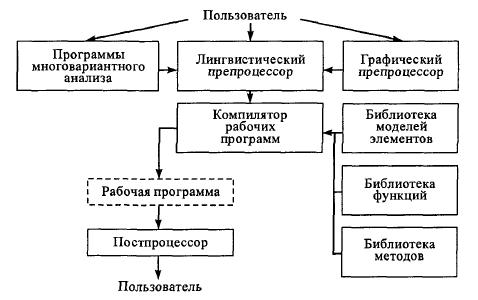
\includegraphics[width=0.6\textwidth]{136.jpg}
\caption{Структура программного комплекса анализа на макроуровне}
\end{figure}

% Вопрос 137 ----------------------------------------------------------
\section{Математическое обеспечение анализа на микроуровне.}

Математическими моделями на микроуровне являются дифференциальные уравнения в частных производных или интегральные уравнения, описывающие поля физических величин. Другими словами, на микроуровне используются модели с распределенными параметрами. В качестве независимых переменных в моделях могут фигурировать пространственные переменные и время.

Характерными примерами моделей могут служить уравнения математической физики вместе с заданными краевыми условиями. Краевые условия включают в себя начальные условия, характеризующие пространственное распределение зависимых переменных в начальный момент времени, и граничные, задающие значения этих переменных на границах рассматриваемой области в функции времени.

В САПР решение дифференциальных или интегро-дифференциальных уравнений с частными производными выполняется численными методами. Эти методы основаны на дискретизации независимых переменных --- их представ-
лении конечным множеством значений в выбранных узловых точках исследуемого пространства. Эти точки рассматриваются как узлы некоторой сетки, поэтому используемые в САПР методы --- это сеточные методы. Среди сеточных методов наибольшее распространение получили два метода: метод конечных разностей (МКР) и метод конечных элементов (МКЭ). Обычно выполняют дискретизацию пространственных независимых переменных, т. е. используют пространственную сетку. В этом случае результатом дискретизации является система обыкновенных диф. уравнений для задачи нестационарной или система алгебраических уравнении для стационарной.

% Вопрос 138 ----------------------------------------------------------
\section{Математическое обеспечение анализа на функционально-логическом уровне.}

На функционально-логическом уровне исследуют устройства, в качестве элементов которых принимают достаточно сложные узлы и блоки, считавшиеся системами на макроуровне, поэтому вместо полных моделей узлов и блоков нужно использовать их макромодели.

В моделях функционально-логического уровня фигурируют переменные одного типа, называемые сигналами. Основой моделирования аналоговых устройств на функционально-логическом уровне является использование аппарата передаточных функций. При этом модель каждого элемента представляют в виде уравнения вход-выход.

Другое упрощающее допущение при моделировании на функционально-логическом уровне --- неучет влияния нагрузки на характеристики блоков. Действительно, подключение к выходу блока некоторого другого узла не влияет на модель блока.

Таким образом, анализ сводится к следующим операциям:
\begin{enumerate}
\item заданную схему устройства представляют совокупностью звеньев, и если схема не полностью покрывается типовыми звеньями, то разрабатывают оригинальные модели;
\item формируют мат. модель системы (ММС) из моделей звеньев;
\item применяют прямое преобразование Лапласа к входным сигналам;
\item решают систему уравнений ММС и находят изображения выходных сигналов;
\item с помощью обратного преобразования Лапласа возвращаются во временную область из области комплексной переменной р.
\end{enumerate}

Анализ дискретных устройств на функционально-логическом уровне требуется прежде всего при проектировании устройств вычислительной техники и цифровой автоматики. Здесь дополнительно к допущениям, принимаемым при анализе аналоговых устройств, используют дискретизацию сигналов, причем базовым является двузначное представление сигналов. Удобно этими двумя
возможными значениями сигналов считать «истину» (иначе 1) и «ложь» (иначе 0), а сами сигналы рассматривать как булевы величины. Тогда для моделирования можно использовать аппарат математической логики. Находят применение также трех- и более значные модели.

% Вопрос 139 ----------------------------------------------------------
\section{Математическое обеспечение анализа на системном уровне.}

Объектами проектирования на системном уровне являются такие сложные системы, как производственные предприятия, транспортные системы, вычислительные системы и сети, автоматизированные системы проектирования и управления и т. п. В этих приложениях анализ процессов функционирования систем связан с исследованием прохождения через систему потока заявок (иначе называемых требованиями или транзактами). Заявками могут быть заказы на производство изделий, задачи, решаемые в вычислительной системе, клиенты в банках, грузы, поступающие на транспортировку, и др. Очевидно, что параметры заявок, поступающих в систему, являются случайными величинами и при проектировании могут быть известны лишь их законы распределения и числовые характеристики этих распределений. Поэтому анализ функционирования на системном уровне, как правило, носит статистический характер. В качестве математического аппарата моделирования удобно принять теорию массового обслуживания, а в качестве моделей систем на этом уровне использовать системы 
массового обслуживания (СМО).

Типичными выходными параметрами в СМО являются числовые характеристики таких величин, как время обслуживания заявок в системе, длины очередей заявок на входах, время ожидания обслуживания в очередях, загрузка устройств системы, а также вероятность обслуживания в заданные сроки и т. п.

В простейшем случае СМО представляет собой некоторое средство, называемое обслуживающим аппаратом (ОА), вместе с очередями заявок на входах. Более сложные СМО состоят из многих взаимосвязанных ОА. Обслуживающие аппараты СМО в совокупности образуют статические объекты СМО, иначе называемые ресурсами. Например, в вычислительных сетях ресурсы представлены аппаратными и программными средствами.

Состояние СМО характеризуется состояниями составляющих ее объектов. Например, состояния ОА выражаются булевыми величинами, значения которых интерпретируются как true (занято) и false (свободно), и длинами очередей на входах ОА.

Правило, согласно которому заявки выбирают из очередей на обслуживание, называют дисциплиной обслуживания, а величину, выражающую преимущественное право на обслуживание, --- приоритетом. В бесприоритетных дисциплинах все транзакты имеют одинаковые приоритеты. Среди бесприоритетных дисциплин наиболее популярны дисциплины FIFO, LIFO и со случайным выбором заявок из очередей.

Системы массового обслуживания отображают процессы с конечным множеством состояний и отсутствием после действия. Такие процессы называют конечными Марковскими цепями.

Марковские цепи характеризуются множеством состояний, матрицей вероятностей перехода из одного состояния в другое и начальное состояние. Марковская цепь представляется в виде графа в котором вершины --- это состояния, а дуги --- вероятности перехода. Основой описания таких систем являются уравнения Колмогорова и сети Петри.


% Вопрос 140 ----------------------------------------------------------
\section{Математическое обеспечение подсистем машинной графики и геометрического моделирования.}

Различают 2D и 3D графику.

2D  графика --- это подготовка документации в машиностроительных САПР и топологическое проектирование печатных плат и кристаллов БИС в САПР электроники.

3D графика применяется для синтеза конструкций, представления траекторий рабочих органов станков при обработке заготовок, генерации сетки конечных элементов при анализе прочности. В 3D-моделировании различают каркасные (проволочные), поверхностные, объемные (твердотельные) модели. 

Каркасная модель представляет собой форму детали в виде конечного множества линий, лежащих на поверхностях детали. Для каждой линии известны координаты концевых точек и указана их инцидентность ребрам или поверхностям. Оперировать каркасной моделью на дальнейших операциях маршрутов проектирования неудобно, и поэтому каркасные модели в настоящее время используют редко.

Поверхностная модель отображает форму детали с помощью задания ограничивающих ее поверхностей, например, в виде совокупности данных о гранях, ребрах и вершинах.

В настоящее время применяются следующие приемы для построения геометрических моделей:

\begin{enumerate}
\item задание граничных элементов: граней ребер, вершин;
\item кинематический подход --- задают траекторию перемещения двумерного контура, след от перемещения принимают в качестве поверхности;
\item позиционный подход --- это пространство разбивают на ячейки и деталь задают с помощью указания этих ячеек.
\item представление сложной детали в виде совокупности базовых элементов форм и выполненных над ними теоретико-множественных операций: пересечение, объединение, разность. Метод базовых элементов формы называется методом конструктивной геометрии, являющейся основным способом конструирования сборочных узлов современных САПР.
\end{enumerate}

Поверхностные модели можно задать следующими формами:

\begin{enumerate}
\item модель состоящая из списка граней, грань представлена списком вершин;
\item метод ребер --- ребра заданы вершинами и гранями.
\end{enumerate}

Наиболее популярным описанием неплоских поверхностей являются кубические уравнения в форме Безье и В-cплайнов.
В подсистемах машинной графики и геометрического моделирования используются параметрически задаваемые кубические кривые:
$$
\left \{ 
\begin{array}{l}
x(t)=a_x t^3 + b_x t^2 + c_x t + d_x\\
y(t)=a_y t^3 + b_y t^2 + c_y t + d_y\\
z(t)=a_z t^3 + b_z t^2 + c_z t + d_z
\end{array} \right.
$$
где $1\geq t\geq 0$.

Такими кривыми описываются сегменты аппроксимируемой кривой. Применение кубических кривых обеспечивает выполнение четырех условий сопряжения сегментов(a, b, c, d). В случае кривых Безье этими условиями являются прохождение кривой сегмента через две заданные концевые точки и равенство в этих точках касательных векторов соседних сегментов.

\end{document}